\documentclass[9pt]{beamer}
\usepackage[ruled, french, onelanguage]{algorithm2e}
\usepackage{tikz}
\usepackage{listings}
\usepackage{hyperref}
\usepackage{amsmath,amssymb,amsfonts}
\usepackage{bm}
\usepackage{xcolor}

\hypersetup{
    colorlinks,
    citecolor=blue,
    filecolor=black,
    linkcolor=blue,
    urlcolor=blue
}

\newcommand{\bbm}[1]{{\mathbf{#1}}}
\DeclareMathOperator*{\argmin}{argmin}   % Jan Hlavacek
\usetheme{Rochester}
\usecolortheme{default}

\beamertemplatenavigationsymbolsempty

\title[exposé]{Construction de modèles réduits pour
des EDPs fortement non-linéaires avec des PINNs}
\author{Vincent Italiano}
\institute{Encadrants: E.Franck (INRIA), V. Michel-Dansac (INRIA), V. Vigon (IRMA) et H. Baty (ObAS)}
\date{Stage de fin de Master}

\begin{document}
\begin{frame}    
    \maketitle

\end{frame}

\begin{frame}
    \frametitle{Contexte du projet}

    \begin{itemize}
        \item Succès des méthodes de deep learning (traitement automatique du langage, computer vision, etc.) \cite{Lecun}.
        \item Peu d'utilisation dans le domaine des méthodes numériques jusqu'à l'arrivée des PINNs \cite{raissi2017physicsI}.
        \item Nécessité d'avoir des modèles réduits (optimisation, analyse de sensibilité, etc.).
        \item \'Etude des phénomènes de reconnection magnétique \cite{Baty_2019}.
    \end{itemize}

\end{frame}

\begin{frame}
    \frametitle{Roadmap}

    \begin{itemize}
        \item Compréhension et prise en main d'un code PINN. \textcolor{green}{\checkmark}
        \item Essais sur l'équation de Burgers en 1D. \textcolor{green}{\checkmark}
        \item Cas test en 2D. \textcolor{green}{\checkmark}
        \item Implémentation de l'échantillonnage préférentiel. \textcolor{green}{\checkmark}
        \item Réduction de modèle sur l'équation de Burgers. \textcolor{green}{\checkmark}
        \item Compréhension et implémentation de la MHD réduite. \textcolor{green}{\checkmark}
        \item Résolution de la MHD avec des PINNs. \textcolor{green}{\checkmark}
        \item Réduction de modèle sur la MHD. \textcolor{red}{$\times$}
    \end{itemize}
\end{frame}

\begin{frame}
    \frametitle{Physics-Informed-Neural-Networks (PINNs)}

    On considère des EDP génériques  

    \begin{align*}
        \mathcal{N}[t,\bbm x, u] &= 0 \quad \text{ dans } ]0,T]\times\Omega\\
        \mathcal{I}[\bbm x, u] &= 0 \quad \text{ dans } \Omega\\      
        \mathcal{B}[t,\bbm x, u] &= 0 \quad \text{ dans } [0,T]\times \partial\Omega
        \label{pde:1}
    \end{align*} 
    sur un domaine $\Omega\in\mathbb{R}^d$ de bord $\partial \Omega$.

    \begin{itemize}
        \item $\mathcal{N}$ est un opérateur differentiel qui représente l'EDP.
        \item $\mathcal{I}$ réprésente la condition initiale.
        \item $\mathcal{B}$  réprésente les contidions aux bords (Dirichlet, Neumann, Robin).
    \end{itemize}

    \begin{exampleblock}{\vspace*{-2ex}}
       
    Un PINN est un réseau de neurones $u_{\bm \theta}$ qui approxime la solution de l'EDP
    ($\bm \theta$ est l'ensemble des paramètres du réseau)
    \end{exampleblock}

\end{frame}

% entrainements + loss 
\begin{frame}[plain]

    Entrainement des PINNs: algorithme de gradient stochastique. On tire de manière uniforme :

    \begin{itemize}
        \item $N_r$ points $\{(t_i^r, x_i^r)\}_{i=1}^{N_r}$ dans $]0,T] \times \Omega$
        \item $N_0$ points $\{(t^0_i,x^0_i)\}_{i=1}^{N_0}$ dans $\{0\} \times \Omega$
        \item $N_b$ points $\{(t^b_i,x^b_i)\}_{i=1}^{N_b} $ dans $]0,T] \times \partial \Omega$
    \end{itemize}

    Puis on minimise la loss 
    \begin{equation*}
        J(\bm \theta)= J_{\mathcal{N}}(\bm \theta) + \lambda_1 J_{\mathcal{I}}(\bm \theta) +\lambda_2 J_{\mathcal{B}}(\bm \theta)
    \end{equation*}
    sur un batch de $m$ points de collocation tirés uniformément à chaque itération.

    \begin{itemize}
        \item MSE sur le résidu de l'EDP
        $$
            J_{\mathcal{N}}(\bm \theta) = \frac{1}{m} \sum_{j=1}^{m} \mathcal{N}[t_j^r,\bbm x_j^r, u_{\bm \theta}(t_j^r,\bbm x_j^r)]^2
        $$
        \item  MSE sur les conditions initiales et conditions aux bords
        $$
            J_{\mathcal{I}}(\bm \theta) =  \frac{1}{N_0} \sum_{j=1}^{N_0} \mathcal{I}[\bbm x_j^0, u_{\bm \theta}(0, \bbm x_j^0)]^2
        \quad \text{ et } \quad 
            J_{\mathcal{B}}(\bm \theta) =  \frac{1}{N_b} \sum_{j=1}^{N_b} \mathcal{B}[t_j^b,\bbm x_j^b, u_{\bm \theta}(t_j^b,\bbm x_j^b)]^2 
        $$
    \end{itemize}
\end{frame}

\begin{frame}[plain]
        \begin{figure}
            \begin{center}
                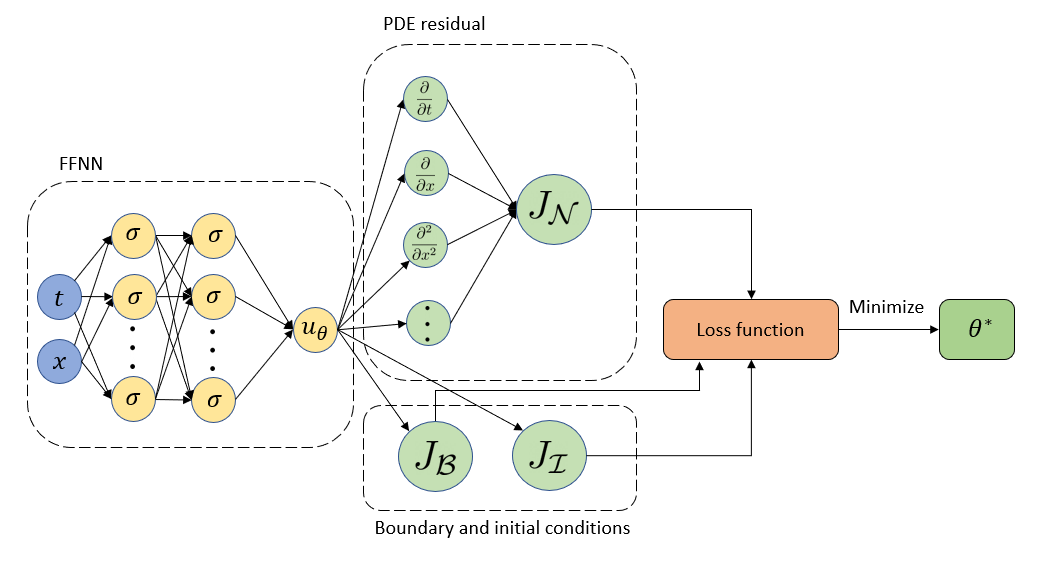
\includegraphics[scale=0.4]{img/coco.png}
            \end{center}
            \caption{Récapitulatif PINNs}
        \end{figure}
\end{frame}


\begin{frame}
    \frametitle{1er exemple : équation de Burgers en 1D}

    1er cas test : $\Omega = [-1,1]$ et $\nu$ est la viscosité

    $$
    \begin{cases}
        \partial_t u + \frac{1}{2}\partial_x u^2 = \nu \partial_{xx}u \quad \text{sur } [0,1]\times\Omega\\
        u(0,x) = \sin(\pi x) \quad \forall x \in \Omega\\
        u(t,-1) = u(t,1) = 0 \quad \forall t \in [0,1]
    \end{cases}
    $$

    \begin{figure}
        \begin{center}
            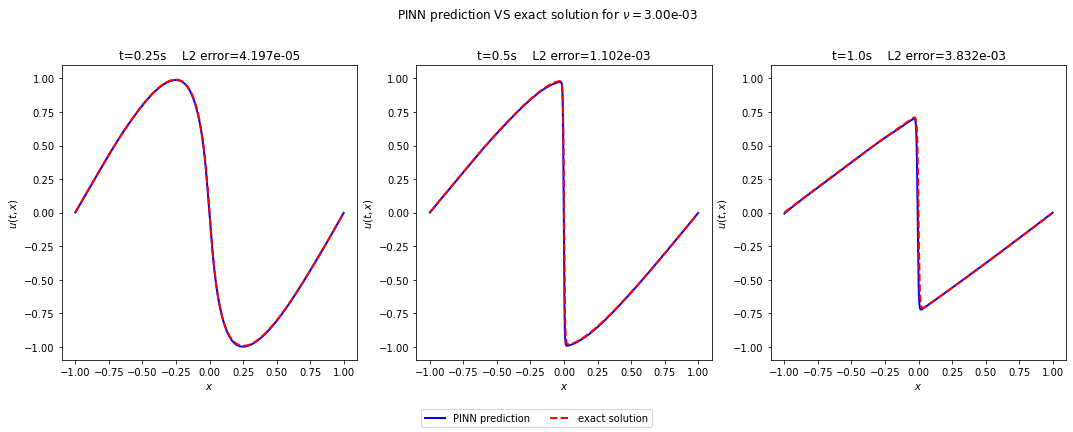
\includegraphics[width=1.\textwidth, height=0.4\textwidth]{img/burgers_nu1.png}
        \end{center}
        \caption{Solution de l'équation de Burgers. Prédiction du PINN vs solution exacte}
    \end{figure}
    
\end{frame}

\begin{frame}[plain]
    
    \begin{figure}
        \begin{center}
            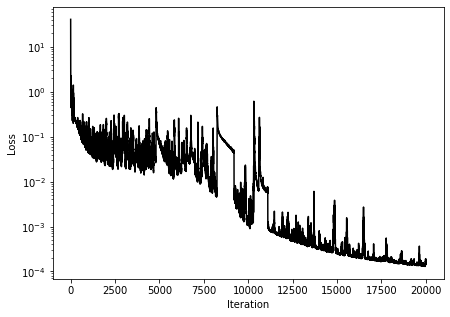
\includegraphics[width=0.49\textwidth,height=0.3\textwidth]{img/burgers_loss1.png}
            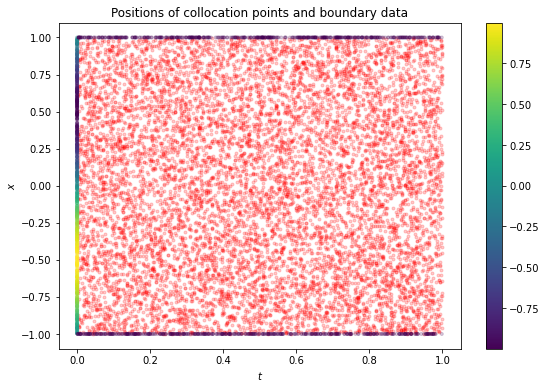
\includegraphics[width=0.49\textwidth,height=0.3\textwidth]{img/burgers_data.png}
        \end{center}
        \caption{\'Evolution de la loss pendant l'entrainement (gauche) répartition des points de collocations (droite)}
    \end{figure}

\end{frame}

%% Burgers 2d
\begin{frame}
    \frametitle{2ème exemple : équation de Burgers 2d}

    EDP en 2 variables d'espace sur le domaine $\Omega = [0,1]\times[0,1]$ et 
    $\nu$ est la viscosité.

    \begin{equation*}
        \begin{cases}
        \partial_t u + \frac{1}{2}\partial_x u^2  + \partial_y u = \nu \Delta u \quad \text{ sur } [0,T] \times \Omega\\
        u(0,x,y) = 1.5-2x \quad \forall (x,y) \in [0,1]\times[0,1]\\
        u(t,0,y) = 1.5, u(t,1,y) = -0.5, u(t,x,0) = 1.5-2x
        \end{cases}
        \label{eq:adv}
    \end{equation*}

\end{frame}


\begin{frame}[plain]
    Résultats numériques : $\nu  = 10^{-3}$, avec un réseau de 8 couches et 150 neurones par couche.
    4h d'entrainement : 
    \begin{figure}
        \begin{center}
            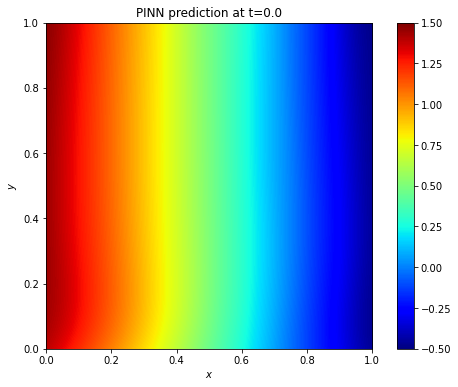
\includegraphics[width=.35\textwidth, height=0.4\textwidth, keepaspectratio]{img/adv_t0.png}
            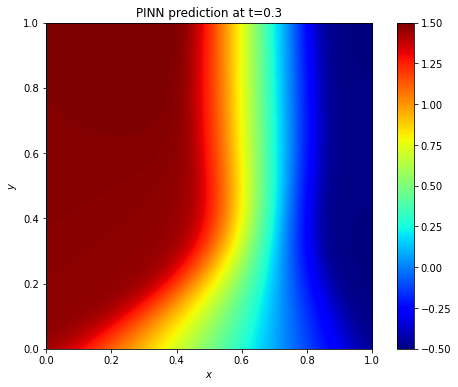
\includegraphics[width=.35\textwidth, height=0.4\textwidth, keepaspectratio]{img/adv_t3.png}
            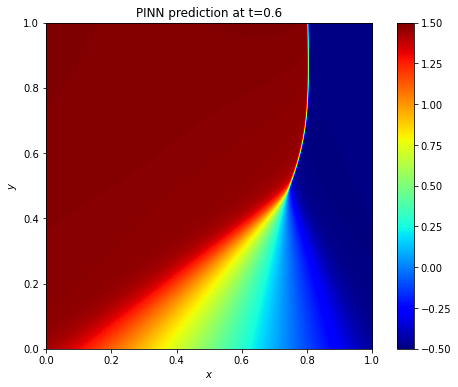
\includegraphics[width=.35\textwidth, height=0.4\textwidth, keepaspectratio]{img/adv_t6.png}
            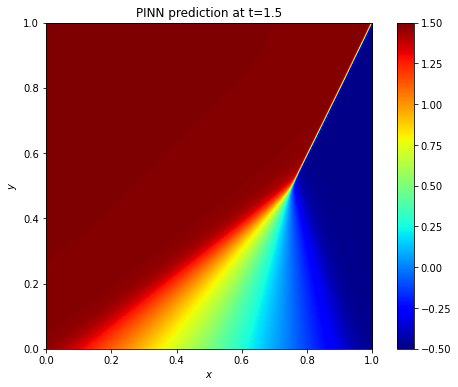
\includegraphics[width=.35\textwidth, height=0.4\textwidth, keepaspectratio]{img/adv_t15.png}
        \end{center}
        \caption{Solution de l'EDP pour $\nu  = 10^{-3}$}
    \end{figure}
    
\end{frame}

\begin{frame}[plain]

   
    \begin{figure}
        \begin{center}
            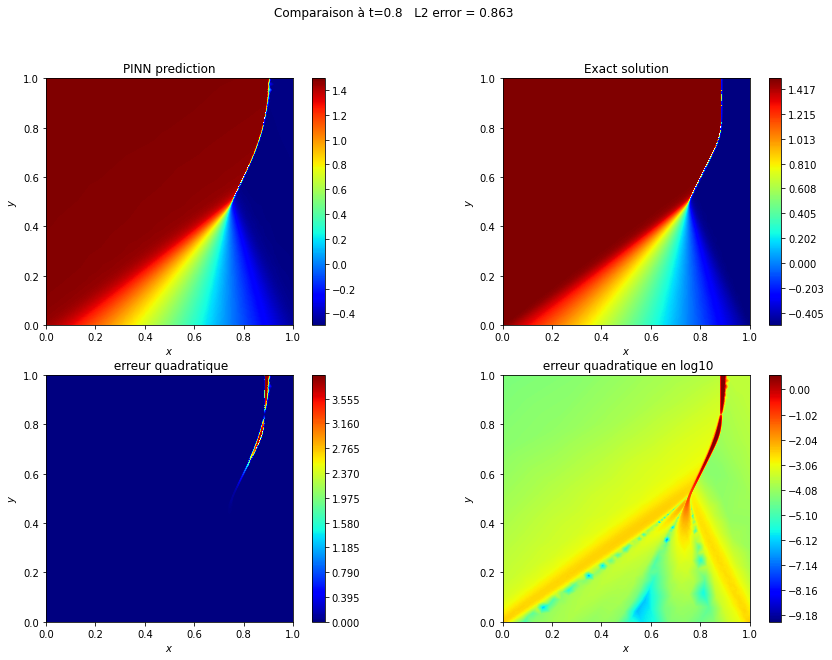
\includegraphics[width=.49\textwidth, keepaspectratio]{img/adv_error2.png}
            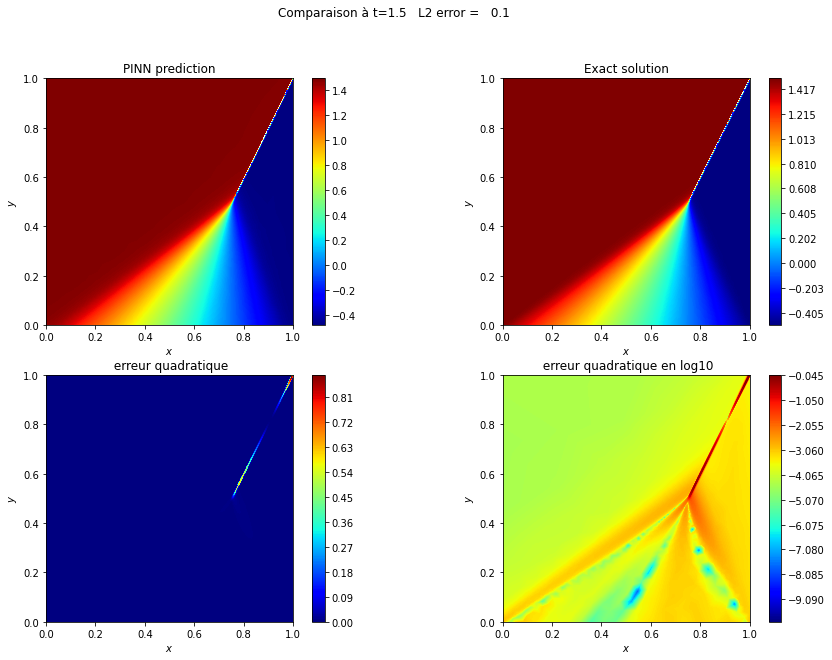
\includegraphics[width=.49\textwidth, keepaspectratio]{img/adv_error.png}
        \end{center}
        \caption{Comparaison avec la solution exacte sur tout le domaine}
    \end{figure}
        
    \begin{figure}
        \begin{center}
            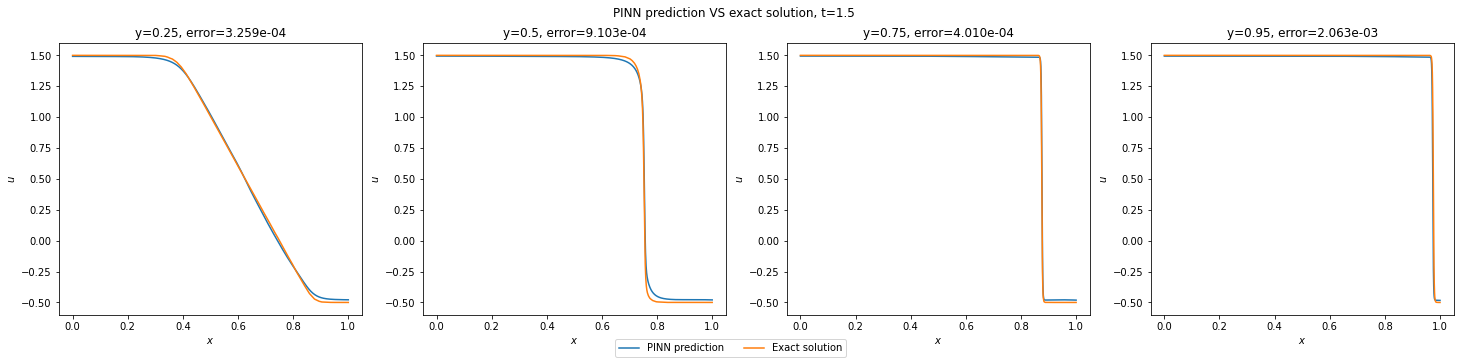
\includegraphics[width=1\textwidth, height=0.4\textwidth, keepaspectratio]{img/adv_slice.png}
        \end{center}
        \caption{Comparaison avec la solution exacte selon des tranches horizontales}
    \end{figure}


\end{frame}

%%%%%%%%%%%%%%%%%%%%%%%%%%%%%%%%%%%%%%%%%%%%%%%%%%%%%%%%%%%%%%%%%%%%%%%%%%%%%%%%%%%%%%%%%%%%%%
% Chapitre 2
%%%%%%%%%%%%%%%%%%%%%%%%%%%%%%%%%%%%%%%%%%%%%%%%%%%%%%%%%%%%%%%%%%%%%%%%%%%%%%%%%%%%%%%%%%%%%%

\begin{frame}
    \frametitle{Echantillonnage préférentiel}

    \begin{block}{\vspace*{-2ex}}
        Idée : modifier le tirage des points utilisés lors de l'entrainement pour accélérer la convergence
    \end{block}

    \vspace*{.5cm}

    Deux critères envisagés : 
    \begin{itemize}
        \item Le résidu : on choisit les points où le résidu est le plus grand.
        \item Un critère spécifique à l'EDP : par exemple choisir les points où l'entropie est la plus grande pour l'équation de Burgers.
    \end{itemize}

    \begin{figure}
        \begin{center}
            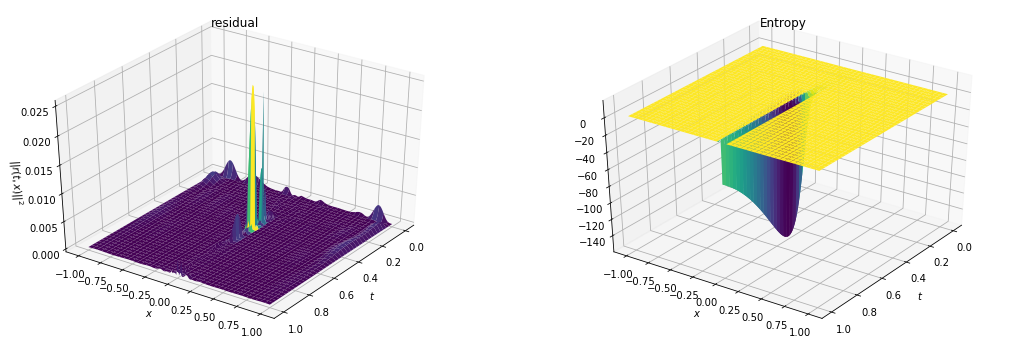
\includegraphics[width=1.\textwidth, height=0.3\textwidth]{img/adaptatif.png}
        \end{center}
        \caption{Résidu (gauche) Entropie (droite) pour une solution de l'équation de Burgers}
    \end{figure}

\end{frame}


\begin{frame}
    \begin{algorithm}[H]
        Générer $N_r$ points de collocation tirés uniformément dans $]0,T]\times\Omega$.\\
        \While{$J(\bm \theta^i)>\varepsilon$}{
            Calculer les probabilités $q_j^i$ selon le critère choisi\\
            Tirer $(1-\alpha) m$ points de collocation selon la loi multinomiale de paramètre $\mathbf{p}^i=(q_j^i)$\\
            Tirer $\alpha m$ points de collocation selon une loi uniforme.\\
            Effectuer la descente de gradient sur le batch obtenu.\\
        }
        \caption{Echantillonage préférentiel}
    \end{algorithm}

    Avec
    \begin{equation}
        q_j^i = \frac{\mathcal{C}(t_j^r, \bbm x_j^r; \bm \theta^i)}{\sum_{j=1}^N \mathcal{C}(t_j^r, \bbm x_j^r; \bm \theta^i)} \quad \forall j=1, \ldots, N_r
    \end{equation}
    où $\mathcal{C}$ désigne le critère choisi (résidu ou entropie).
    
\end{frame}

\begin{frame}[plain]

    Le temps d'entrainement avec un échantillonage préférentiel est plus long (évaluation de la loss en chaque points) 
    mais permet de converger plus vite (en itérations).

    \begin{figure}
        \begin{center}
            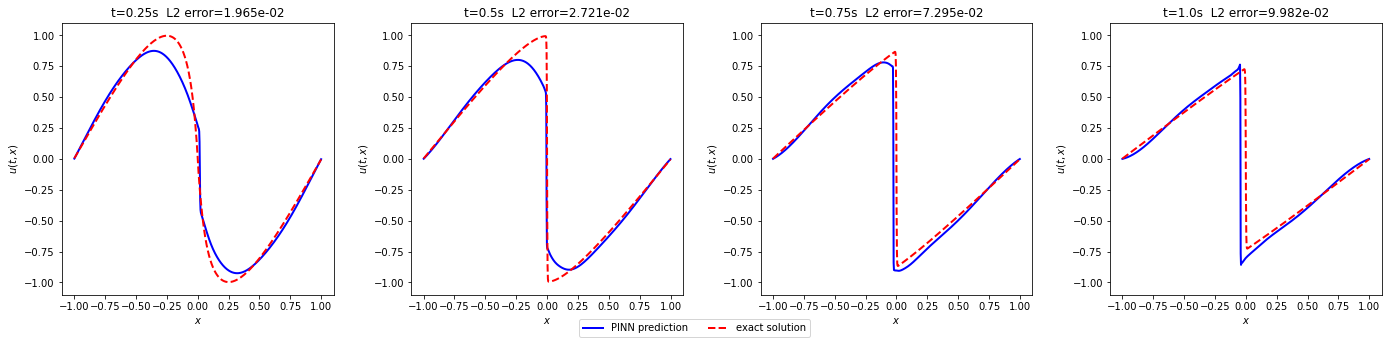
\includegraphics[width=.7\textwidth, height=0.4\textwidth, keepaspectratio]{img/adapt_uniforme1.png}
            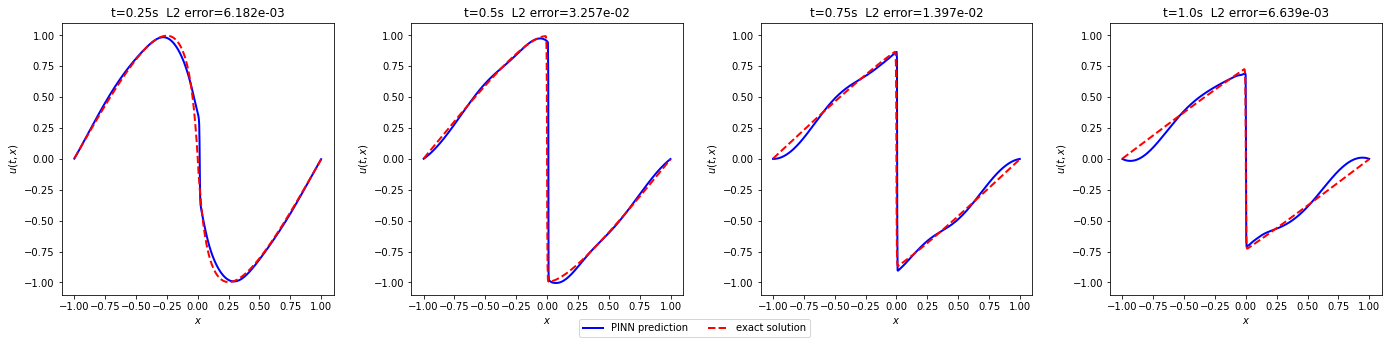
\includegraphics[width=.7\textwidth, height=0.4\textwidth, keepaspectratio]{img/adapt_residu1.png}
        \end{center}
        \caption{Comparaison précision du PINN sur une viscosité faible $\nu=10^{-4}$.
        Avec un tirage uniforme (haut) avec un tirage préférentiel selon le résidu (bas)}
    \end{figure}
   
    Il devient inutile lorsqu'on a beaucoup de points de collocations.
\end{frame}

\begin{frame}
    \frametitle{Modèle réduit pour l'équation de Burgers 1d}
    \begin{columns}
        \begin{column}{0.4\textwidth}

            \vspace*{-1.5cm}
            \begin{block}{\vspace*{-2ex}}
                Idée : Les PINNs sont peu sensibles à la dimension.
            On considère la viscosité comme une variable, on obtient un problème à 3 variables $(t, \bbm x, \nu)$.
            \end{block}
            \vspace*{-.1cm}

            \begin{itemize}
                \item Réseau de taille 16 couches et 256 neurones par couche.
                \item 2h d'entrainement ($\simeq$ autant de temps que pour juste $\nu = 10^{-4}$)
                \item Plage de viscosité allant de $10^{-2}$ à $10^{-4}$
                \item Loss finale obtenue: $10^{-5}$
            \end{itemize}
        \end{column}
        \begin{column}{0.6\textwidth}  %%<--- here
            \begin{figure}
                \begin{center}
                    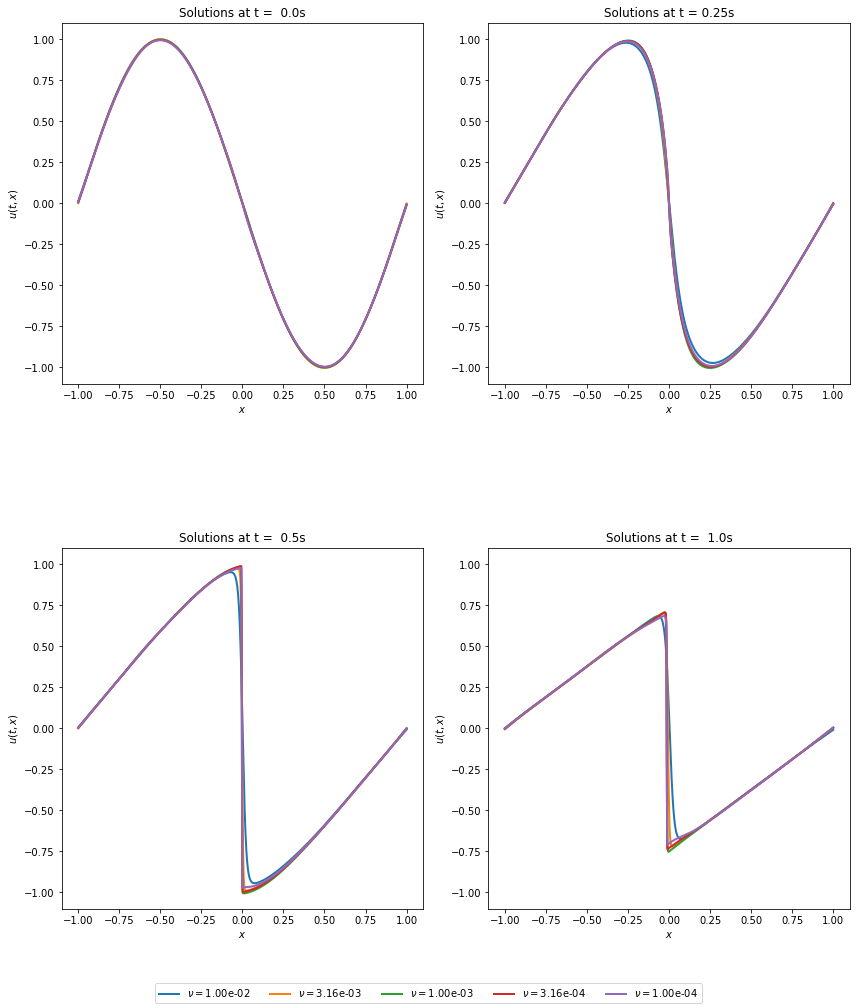
\includegraphics[scale=0.2]{img/burgers_bg.png}
                 \end{center}
                 \caption{Prédiction du PINN pour plusieurs viscosités}
            \end{figure}
        \end{column}
        \end{columns}

\end{frame}

\begin{frame}

    \begin{figure}
        \begin{center}
            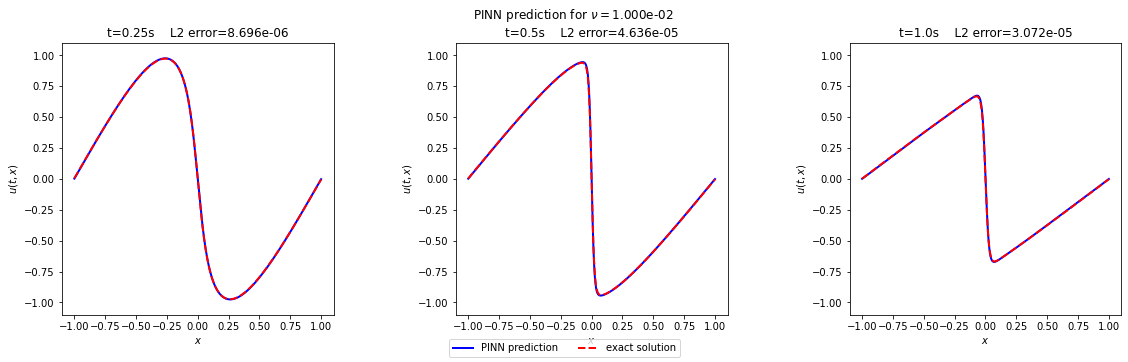
\includegraphics[width=.49\textwidth, height=0.4\textwidth, keepaspectratio]{img/burgers_multi1.png}
            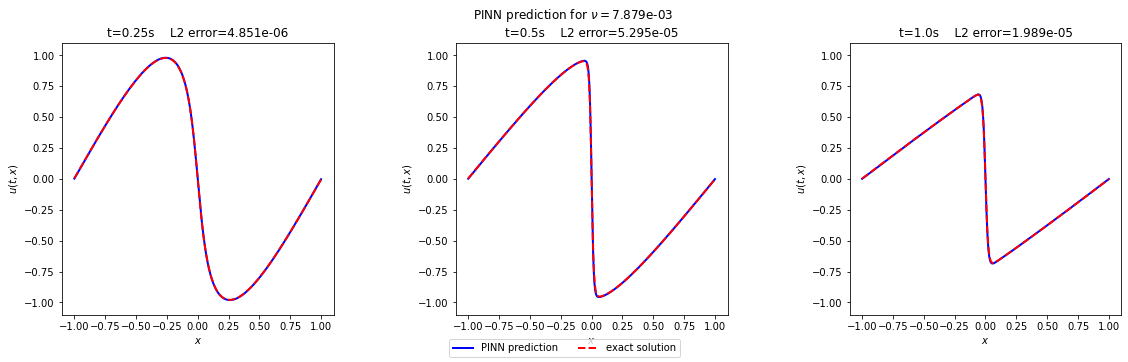
\includegraphics[width=.49\textwidth, height=0.4\textwidth, keepaspectratio]{img/burgers_multi2.png}
            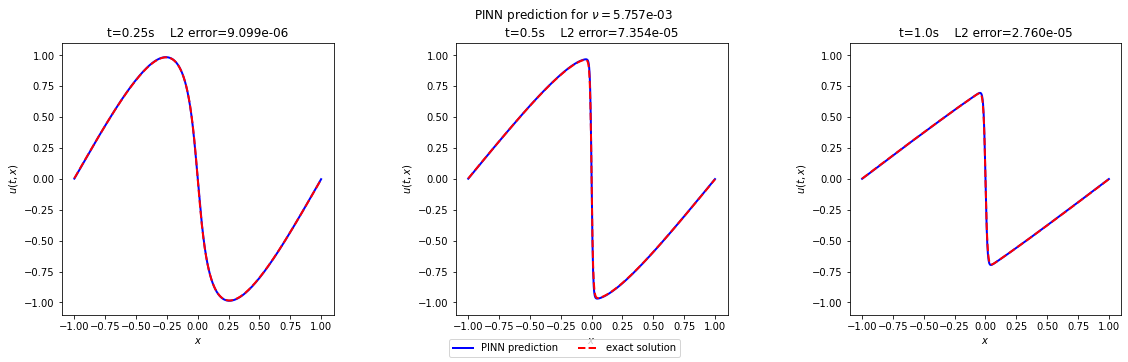
\includegraphics[width=.49\textwidth, height=0.4\textwidth, keepaspectratio]{img/burgers_multi3.png}
            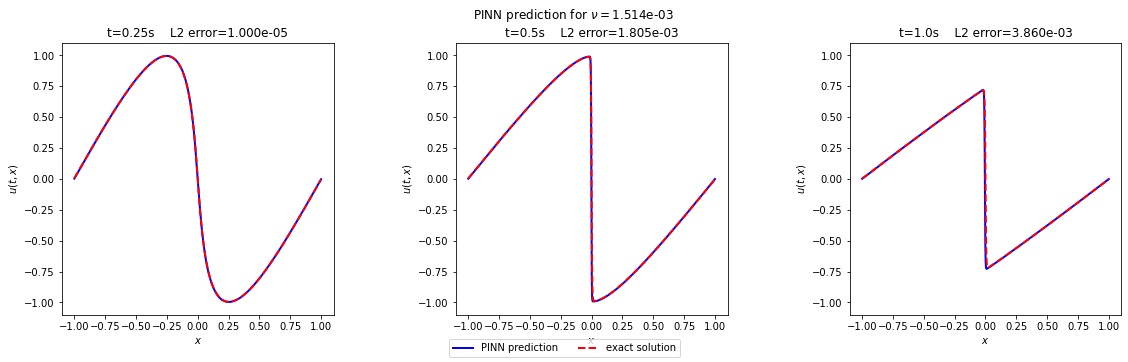
\includegraphics[width=.49\textwidth, height=0.4\textwidth, keepaspectratio]{img/burgers_multi4.png}
            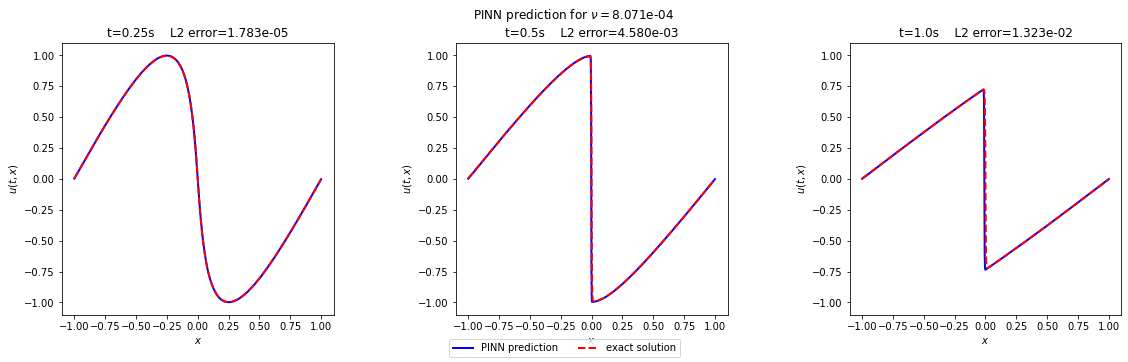
\includegraphics[width=.49\textwidth, height=0.4\textwidth, keepaspectratio]{img/burgers_multi5.png}
            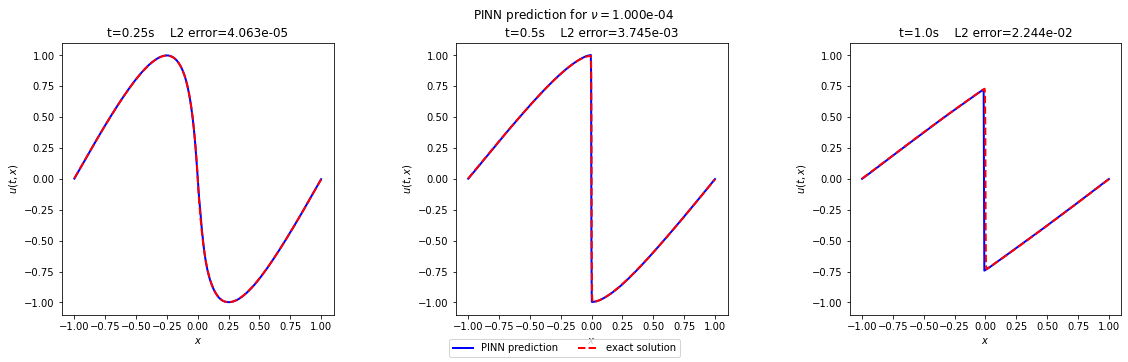
\includegraphics[width=.49\textwidth, height=0.4\textwidth, keepaspectratio]{img/burgers_multi6.png}
        \end{center}
    \caption{Comparaison prédiction du PINN vs solution exacte pour plusieurs viscosités}
    \end{figure}
    
\end{frame}


%%%%%%%%%%%%%%%%%%%%%%%%%%%%%%%%%%%%%%%%%%%%%%%%%%%%%%%%%%%%%%%%%%%%%%%%%%%%%%%%%%%%%%%%%%%%%%
% Chapitre 3 : MHD
%%%%%%%%%%%%%%%%%%%%%%%%%%%%%%%%%%%%%%%%%%%%%%%%%%%%%%%%%%%%%%%%%%%%%%%%%%%%%%%%%%%%%%%%%%%%%%

\begin{frame}
    \frametitle{Application à la magnétohydrodynamique}

    Magnétohydrodynamique (MHD) =  dynamique des fluides conducteurs du courant électrique 
    en présence de champs électromagnétiques (plasmas).

    $$
        \begin{cases}
            \partial_t \rho+ \nabla \cdot (\rho V)= 0 \\
            \partial_t V + (V \cdot \nabla)V = \frac{J\times B - \nabla P}{\rho} + \nu\Delta V \\
            \partial_t B = \nabla \times (V\times B - J) \\
            \partial_t P + V\cdot \nabla P = -\Gamma P \nabla\cdot V
        \end{cases}
    $$
    avec $J = \nabla \times B$ et $\nabla \cdot B = 0$. 
    \vspace*{.5cm}

    $B$ est le champ magnétique, $J$ le courant, $V$ la vitesse du fluide, $\rho$ sa densité, $P$ sa pression, $\nu$ sa viscosité, 
    et $\Gamma$ le coefficient adiabatique.
    
\end{frame}

\begin{frame}
    \frametitle{MHD réduite}

    Modèle réduit de la MHD : fluide incompréssible, dynamique restreinte à un plan, 
    avec viscosité $\nu$ et résistivité $\eta$ uniformes et $\rho=\mu_0=1$.
    \vspace*{.5cm}

    Les équations se réduisent à un système de 4 variables scalaires
    $$
    \begin{cases}
        \partial_t \omega + (V \cdot \nabla) \omega = (B \cdot \nabla)J + \nu\Delta \omega \\
        \partial_t \psi + (V \cdot \nabla)\psi = \eta \Delta \psi \\
        \Delta \phi = - \omega \\
        \Delta \psi = - J
    \end{cases}
    $$

    \vspace*{.5cm}

    $\omega$ est la vorticité et $\psi$ le potentiel vecteur du champ magnétique

\end{frame}

%%%%%%%%%%%%
% Desription du tilt

\begin{frame}
    \frametitle{Instabilité de tilt}

    Configuration d'équilibre intiale :  $\omega_e = \phi_e = 0$ 

    \begin{equation*}
        \psi_e(x,y) = \begin{cases}
            (\frac{1}{r}-r)\frac{y}{r} & \text{si r} > 1\\
            -\frac{2}{kj_0(k)}j_1(kr)\frac{y}{r} & \text{si r} \leq 1
        \end{cases}
        \quad \quad
        J_e(x,y) = \begin{cases}
            0 & \text{si r} > 1\\
            -\frac{2k}{j_0(k)}j_1(kr)\frac{y}{r} & \text{si r} \leq 1
        \end{cases}
    \end{equation*}

    avec $r=\sqrt{x^2+y^2}$, $j_0$ et $j_1$ les première et seconde fonctions de Bessel de première espèce et $k=3.83170597$

    \begin{figure}
        \begin{center}
            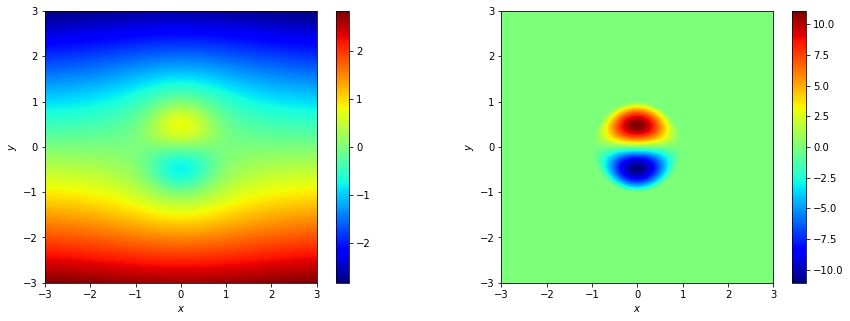
\includegraphics[width=.8\textwidth, height=0.4\textwidth, keepaspectratio]{img/tilt0.png}
        \end{center}
        \caption{Configuration intiale :  $\psi_e$ à gauche et $J_e$ à droite}
    \end{figure}
\end{frame}

\begin{frame}

    \begin{figure}[h!]
        \centering
            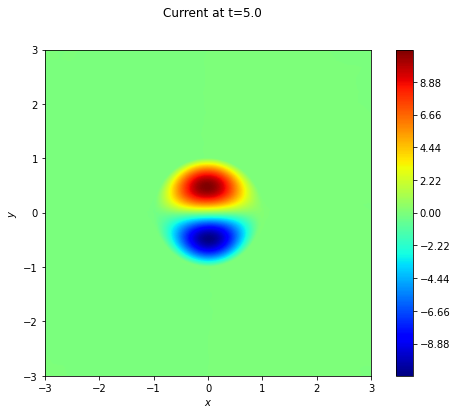
\includegraphics[width=.3\textwidth, height=0.4\textwidth, keepaspectratio]{img/tilt5.png}
            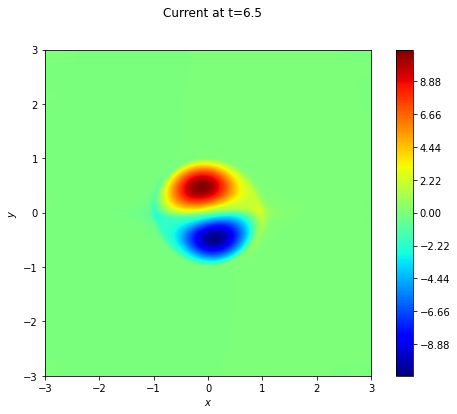
\includegraphics[width=.3\textwidth, height=0.4\textwidth, keepaspectratio]{img/tilt6.png}
            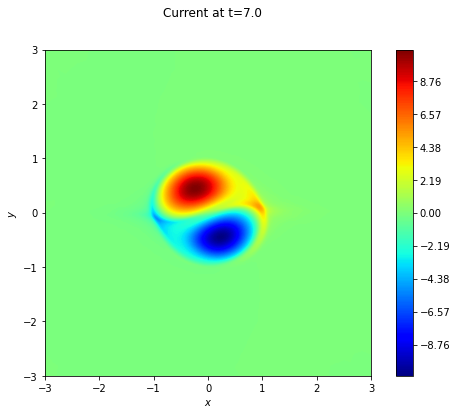
\includegraphics[width=.3\textwidth, height=0.4\textwidth, keepaspectratio]{img/tilt7.png}
            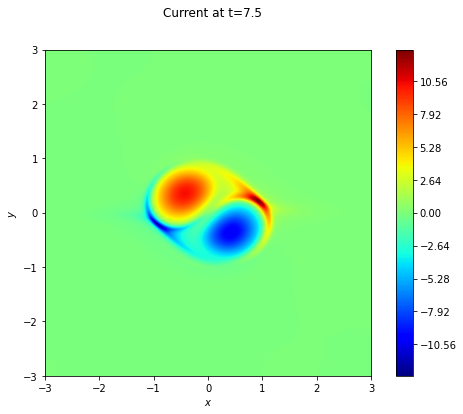
\includegraphics[width=.3\textwidth, height=0.4\textwidth, keepaspectratio]{img/tilt75.png}
            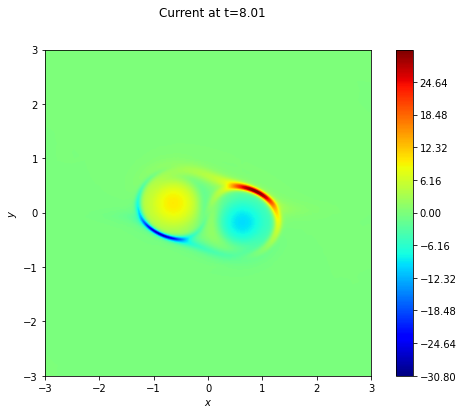
\includegraphics[width=.3\textwidth, height=0.4\textwidth, keepaspectratio]{img/tilt8.png}
            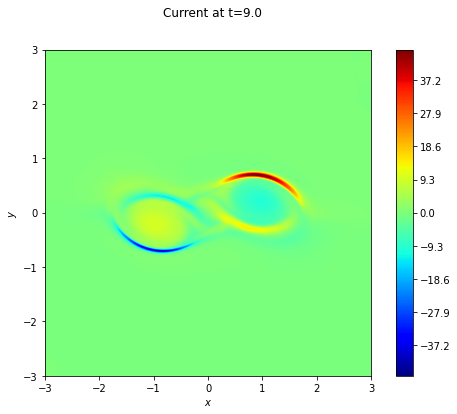
\includegraphics[width=.3\textwidth, height=0.4\textwidth, keepaspectratio]{img/tilt9.png}
            \caption{\'Evolution du courant $J$ durant le développement de l'instabilité de tilt pour 
                une résistivité $\eta = 3\times 10^{-3}$.}
        \label{fig:tilt1}
    \end{figure}

\end{frame}

\begin{frame}
    \frametitle{Résolution}

    \begin{alertblock}{\vspace*{-2ex}}
        Difficulté : problème multi-échelle où les solutions prennent des formes complexes
    \end{alertblock}

    \begin{itemize}
        \item Modification de la loss pour intégrer des données
        \begin{align*}
            J(\bm \theta) =  \frac{1}{m} \sum_{j=1}^{m} \mathcal{N}[t_j^r,\bbm x_j^r, u_{\bm \theta}(t_j^r,\bbm x_j^r)]^2
            + \underbrace{\frac{\lambda}{N_d} \sum_{j=1}^{N_d} \Big[ u_j^d  - u_{\bm \theta}(t_j^d, \bbm x_j^d) \Big]^2}_{ = J_{\text{data}}(\bm \theta)}
            \label{eq:LOSSMHD}
        \end{align*}
        \item On utilise plusieurs snapshots pour guider l'apprentissage
        \item Plusieurs réseaux de neurones composent le PINNs
    \end{itemize}
    \vspace*{.5cm}

    Cela augmente beaucoup le nombre d'hyperparamètres à régler.

\end{frame}

\begin{frame}[plain]

    \begin{itemize}
        \item résistivité $\eta = \nu = 3\times 10^{-3}$
        \item 2 réseaux de 16 couches et 256 neurones par couche.
        \item 10 snapshots (donc 44 hyperparamètres pour l'équilibrage de la loss)
        \item 4h d'entrainement
    \end{itemize}


    \begin{figure}[h!]
        \centering
        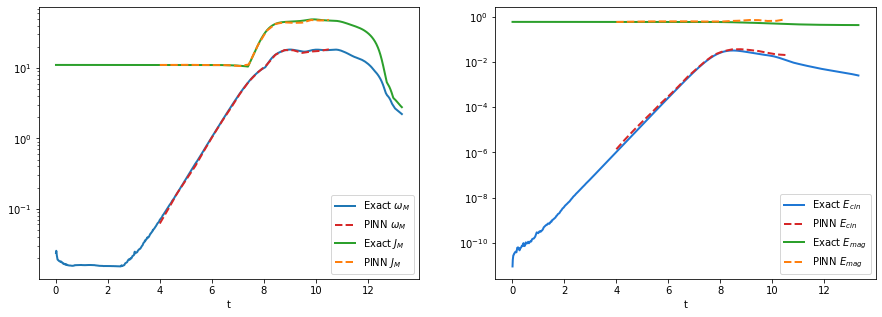
\includegraphics[width=.9\textwidth, keepaspectratio]{img/courbeMHD.png}
        \caption{Prédiction PINNs vs solutione référence : amplitude de courant et de vorticité maximale (gauche) énergie 
        cinétique et magnétique du système
        (droite)}
        \label{fig:tilt3}
    \end{figure}

\end{frame}

\begin{frame}[plain]
    \begin{figure}[h!]
        \centering
            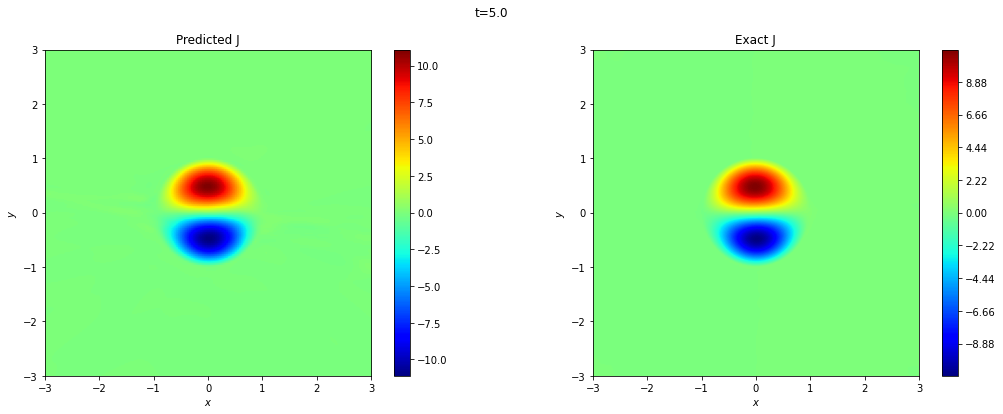
\includegraphics[width=.49\textwidth, height=0.4\textwidth, keepaspectratio]{img/tiltfinal_5.png}
            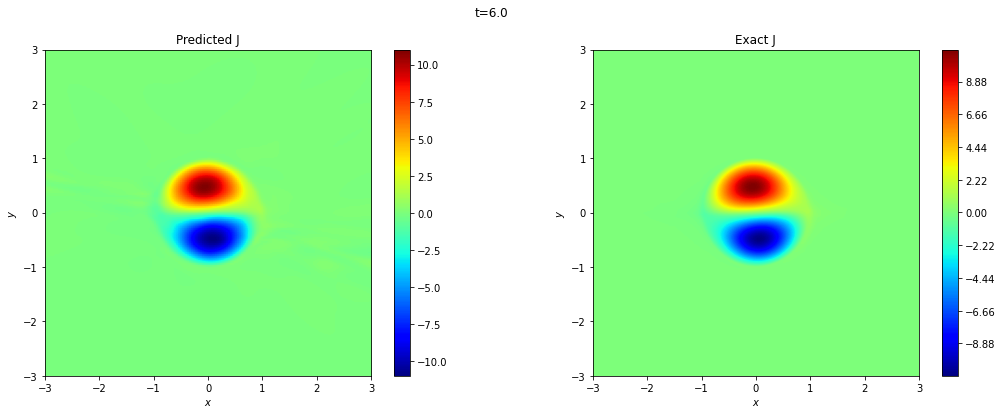
\includegraphics[width=.49\textwidth, height=0.4\textwidth, keepaspectratio]{img/tiltfinal_6.png}
            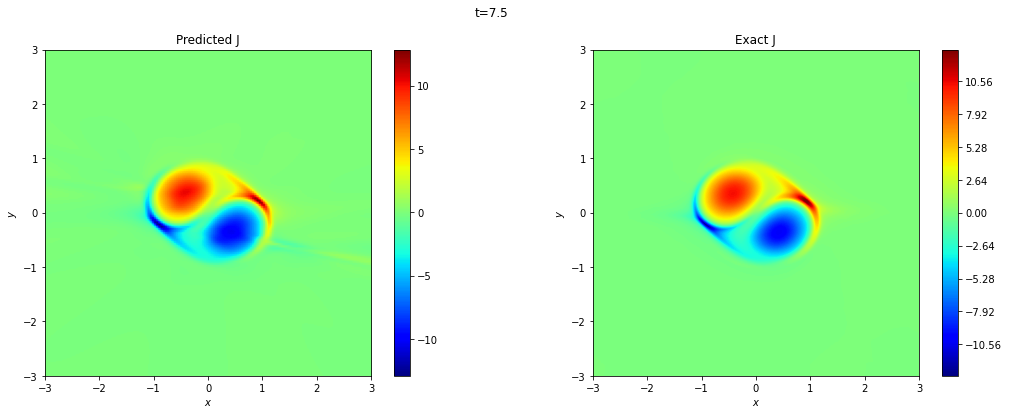
\includegraphics[width=.49\textwidth, height=0.4\textwidth, keepaspectratio]{img/tiltfinal_7.5.png}
            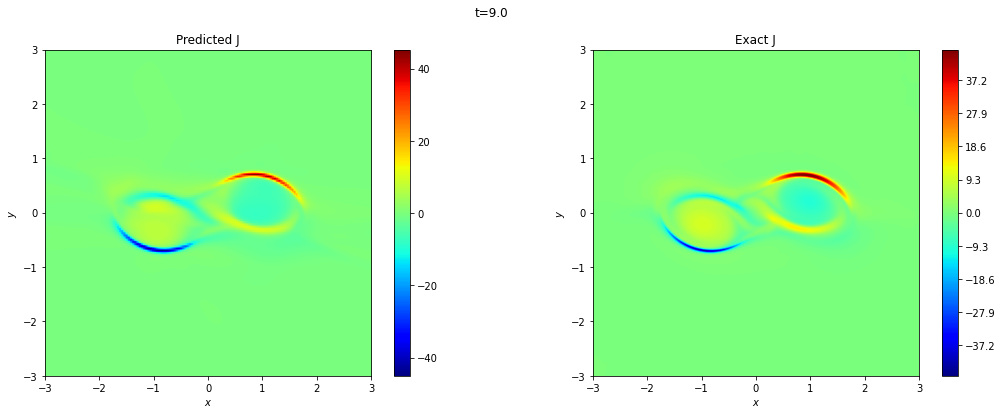
\includegraphics[width=.49\textwidth, height=0.4\textwidth, keepaspectratio]{img/tiltfinal_9.png}
            \caption{Comparaison du courant $J$ prédit par les PINNs vs la solution de référence}
    \end{figure}
\end{frame}

\begin{frame}[plain]
    \begin{figure}
        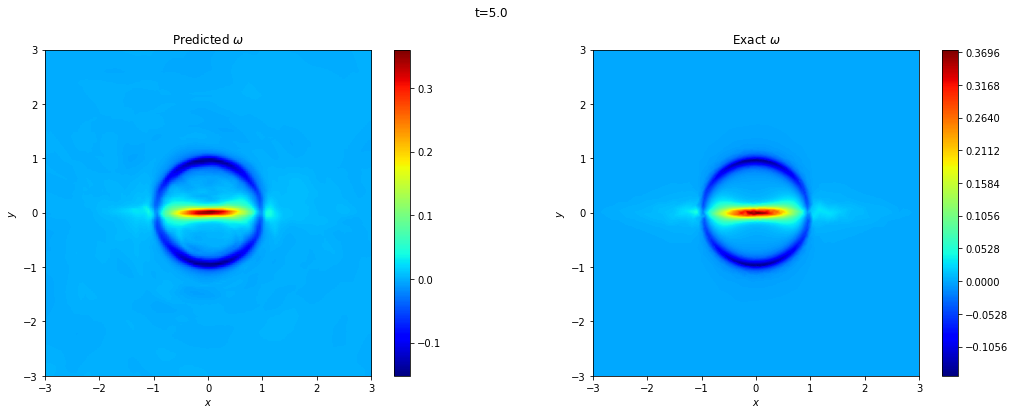
\includegraphics[width=.49\textwidth, height=0.4\textwidth, keepaspectratio]{img/tiltfinalO_5.png}
        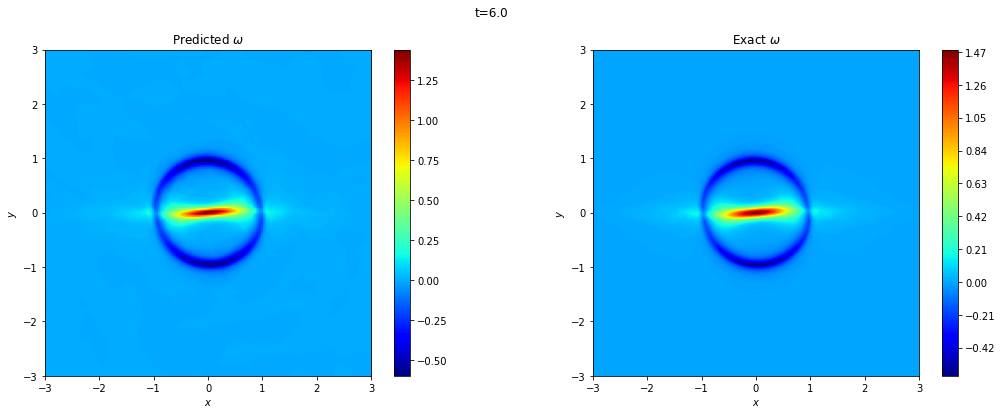
\includegraphics[width=.49\textwidth, height=0.4\textwidth, keepaspectratio]{img/tiltfinalO_6.png}
        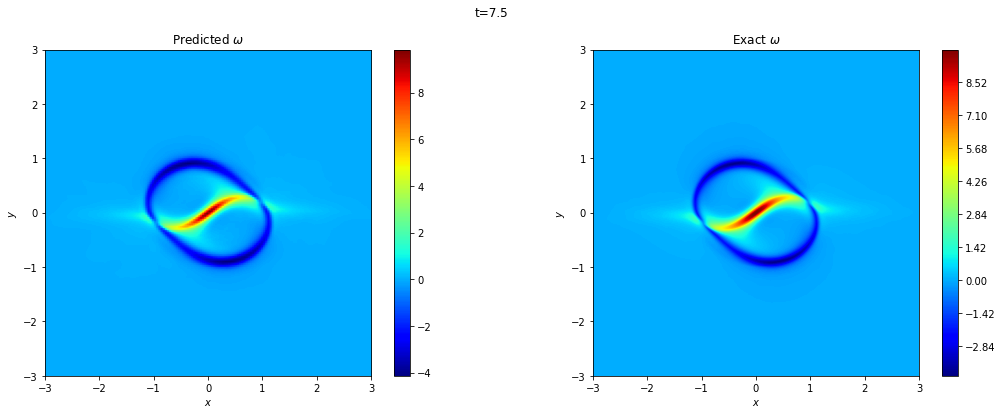
\includegraphics[width=.49\textwidth, height=0.4\textwidth, keepaspectratio]{img/tiltfinalO_7.5.png}
        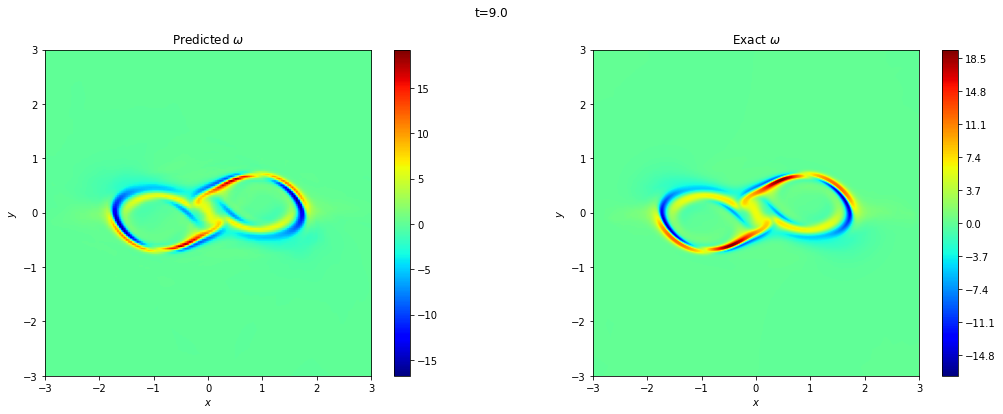
\includegraphics[width=.49\textwidth, height=0.4\textwidth, keepaspectratio]{img/tiltfinalO_9.png}
        \caption{Comparaison de la vorticité $\omega$ prédite par les PINNs vs la solution de référence}
    \end{figure}
\end{frame}

\begin{frame}[plain]
    \begin{figure}
        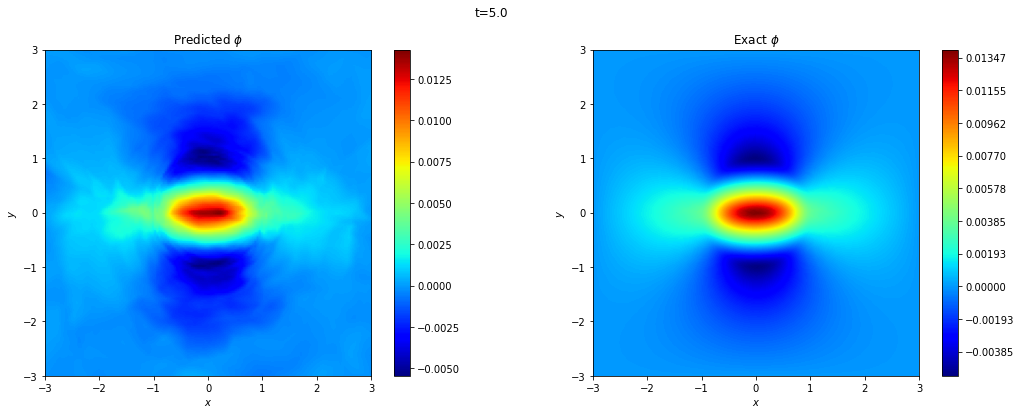
\includegraphics[width=.49\textwidth, height=0.4\textwidth, keepaspectratio]{img/tiltfinalPHI_5.png}
        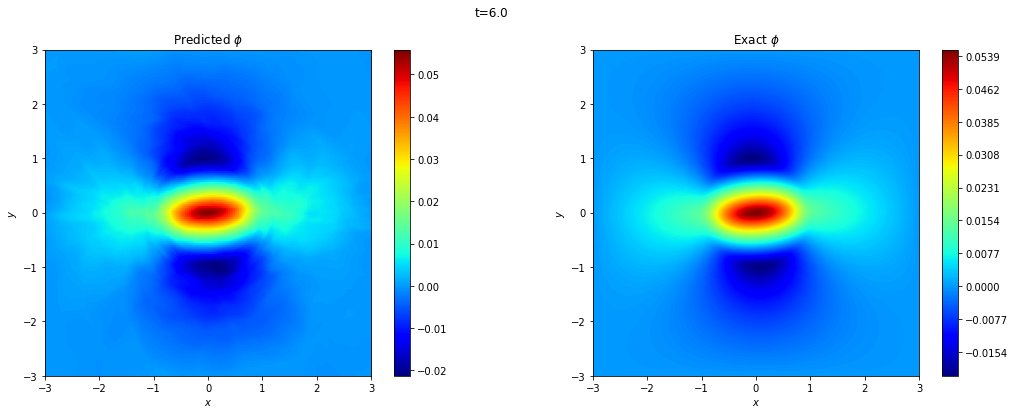
\includegraphics[width=.49\textwidth, height=0.4\textwidth, keepaspectratio]{img/tiltfinalPHI_6.png}
        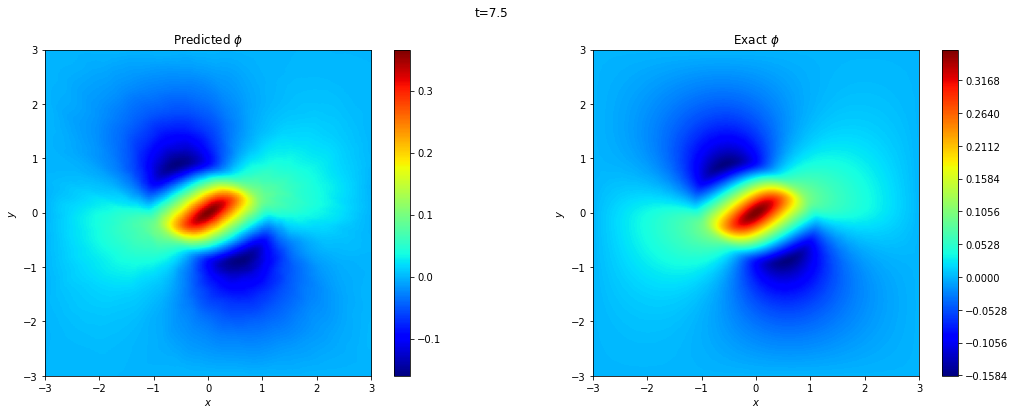
\includegraphics[width=.49\textwidth, height=0.4\textwidth, keepaspectratio]{img/tiltfinalPHI_7.5.png}
        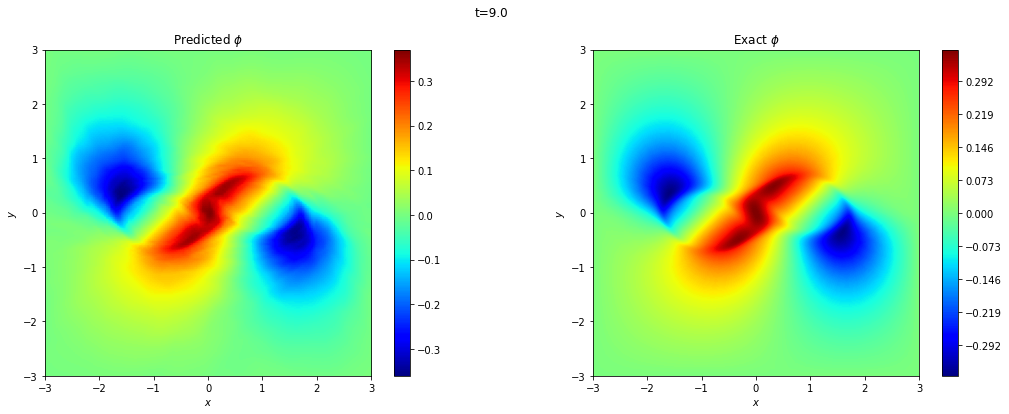
\includegraphics[width=.49\textwidth, height=0.4\textwidth, keepaspectratio]{img/tiltfinalPHI_9.png}
        \caption{Comparaison de la fonction $\phi$ prédite par les PINNs vs la solution de référence}
    \end{figure}
\end{frame}

\begin{frame}[plain]
    \begin{figure}
        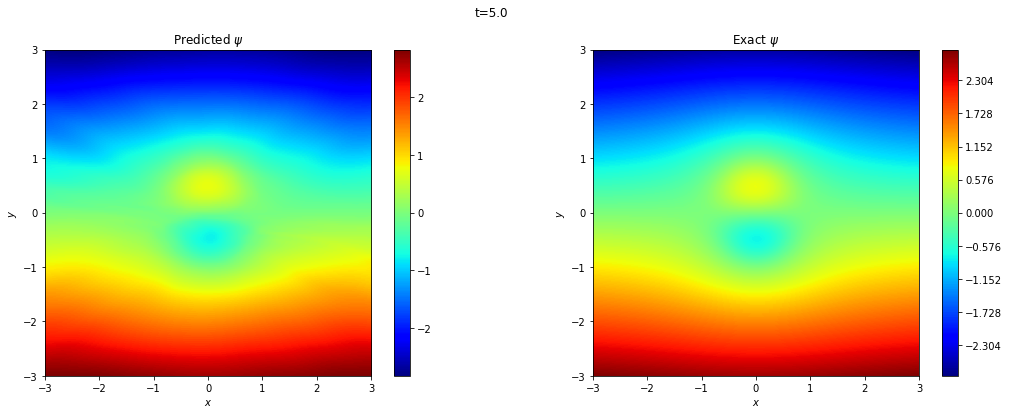
\includegraphics[width=.49\textwidth, height=0.4\textwidth, keepaspectratio]{img/tiltfinalPSI_5.png}
        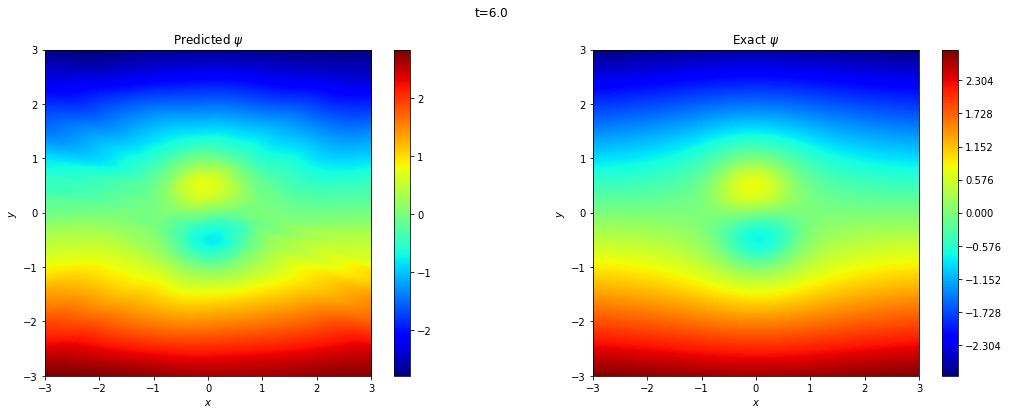
\includegraphics[width=.49\textwidth, height=0.4\textwidth, keepaspectratio]{img/tiltfinalPSI_6.png}
        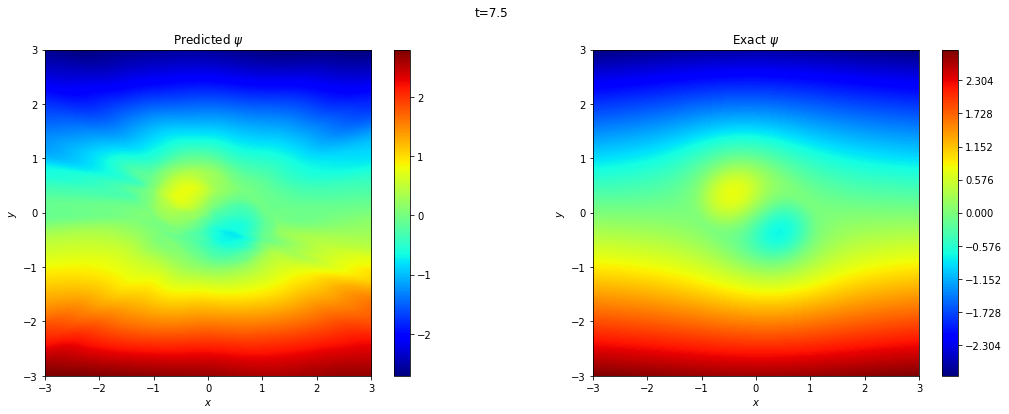
\includegraphics[width=.49\textwidth, height=0.4\textwidth, keepaspectratio]{img/tiltfinalPSI_7.5.png}
        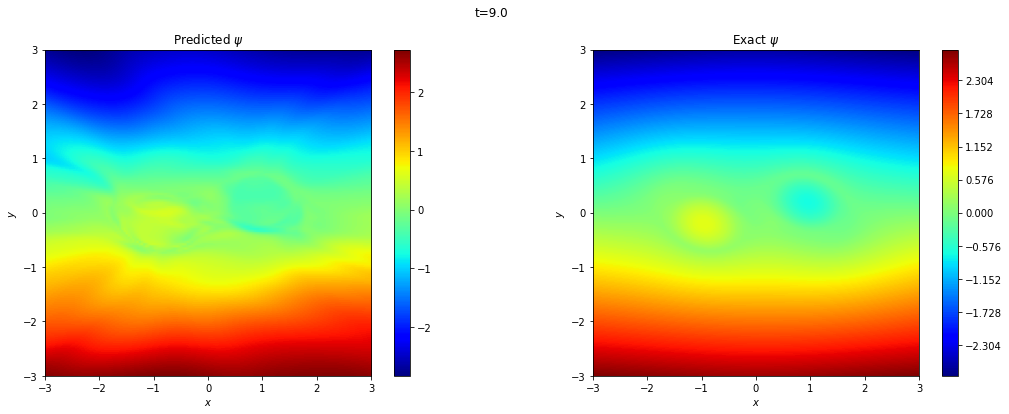
\includegraphics[width=.49\textwidth, height=0.4\textwidth, keepaspectratio]{img/tiltfinalPSI_9.png}
        \caption{Comparaison de la fonction $\psi$ prédite par les PINNs vs la solution de référence}
    \end{figure}
\end{frame}
   

\begin{frame}
    \frametitle{Conclusion}

    \begin{itemize}
        \item Les PINNs peuvent résoudre des EDPs complexes sans maillage
        \item Difficulté pour les systèmes multi-échelle
        \item Entrainement nécsssite de régler beaucoup d'hyperparamètres
    \end{itemize}
    
\end{frame}


\nocite{*}
\begin{frame}[allowframebreaks]
    \frametitle{Bibliographie}

    \bibliographystyle{apalike}
    {\footnotesize
    \bibliography{diapo}}

\end{frame}


\end{document}